\usetikzlibrary{patterns,decorations.pathreplacing}
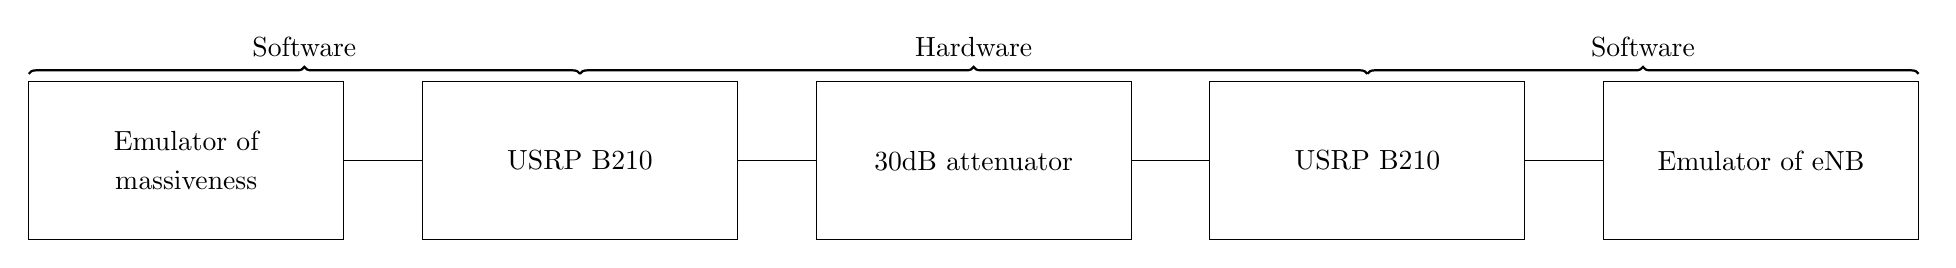
\begin{tikzpicture}
\draw  (-7.5,-1) rectangle (-3.5,-3);
\node at (-5.5,-2) {30dB attenuator};
\draw  (-2.5,-1) rectangle (1.5,-3);
\draw  (-12.5,-1) rectangle (-8.5,-3);
\draw  (-17.5,-1) rectangle (-13.5,-3);
\draw  (2.5,-1) rectangle (6.5,-3);
\node at (-0.5,-2) {USRP B210};
\node at (-10.5,-2) {USRP B210};
\node at (-15.5,-1.75) {Emulator of};
\node at (4.5,-2) {Emulator of eNB};
\node at (-15.5,-2.25) {massiveness};
\draw (-13.5,-2) -- (-12.5,-2);
\draw (-8.5,-2) -- (-7.5,-2);
\draw (-3.5,-2) -- (-2.5,-2);
\draw (1.5,-2) -- (2.5,-2);
\draw [thick,decoration={brace,mirror,raise=0.1cm},decorate] (-10.5,-1) node (v1) {} -- (-17.5,-1) node [pos=0.5,anchor=north,yshift=0.7cm] {Software}; 
\draw [thick,decoration={brace,mirror,raise=0.1cm},decorate] (6.5,-1) node (v1) {} -- (-0.5,-1) node [pos=0.5,anchor=north,yshift=0.7cm] {Software}; 
\draw [thick,decoration={brace,mirror,raise=0.1cm},decorate] (-0.5,-1) node (v1) {} -- (-10.5,-1) node [pos=0.5,anchor=north,yshift=0.7cm] {Hardware}; 
\end{tikzpicture}